% !TeX root = RJwrapper.tex
\title{\pkg{langevitour}: Smooth Interactive Touring of High Dimensions, Demonstrated with scRNA-Seq Data}


\author{by Paul Harrison}

\maketitle

\abstract{%
\CRANpkg{langevitour} displays interactive animated 2D projections of high-dimensional datasets.
Langevin Dynamics is used to produce a smooth path of projections. Projections are initially explored at random. A ``guide'' can be activated to look for an informative projection, or variables can be manually positioned. After a projection of particular interest has been found, continuing small motions provide a channel of visual information not present in a static scatter plot.
\CRANpkg{langevitour} is implemented in Javascript, allowing for a high frame rate and responsive interaction, and can be used directly from the R environment or embedded in HTML documents produced using R.
Single cell RNA-sequencing (scRNA-Seq) data is used to demonstrate the widget. \CRANpkg{langevitour}'s linear projections provide a less distorted view of this data than commonly used non-linear dimensionality reductions such as UMAP.
}

\hypertarget{introduction}{%
\section{Introduction}\label{introduction}}

Understanding high-dimensional data is difficult. High-dimensional data is data where many variables have been measured at once. There may be complex relationships between variables, and the data may contain clusters and other features with complex shapes. This article introduces a new interactive tool that may be helpful for visualizing and understanding high-dimensional data using animated 2D projections.

High-dimensional data is produced in fields across the breadth of science. This article will focus on a motivating example from biology. Single cell RNA-sequencing (scRNA-Seq) typically measures the expression levels of thousands of genes in tens of thousands of biological cells. We can think of cells as points in a gene-expression space with thousands of dimensions. There is a complex high-dimensional geometry due to differences between biological cell types, variation in expression within cell types, cell developmental trajectories, and treatment responses. Principal Components Analysis (PCA) can find a set of directions in which the data is most variable, allowing scRNA-Seq data to be summarized down to perhaps tens of dimensions while still capturing most of the important geometry. However even a ten-dimensional space is difficult to comprehend.

One way to explore high-dimensional data is using a ``tour.'' A tour is a sequence of projections of the dataset, most commonly into two dimensions. A Grand Tour (Asimov 1985) is a tour that will eventually visit as close as we like to every possible projection of the data, typically using a sequence of random projections. A Guided Tour, on the other hand, seeks an ``interesting'' projection by moving toward the maximum of some index function (Cook et al. 1995). The sequence of projections is animated, with smooth interpolation between each successive pair of projections. The software XGobi and GGobi (Swayne, Cook, and Buja 1998) provide an interactive graphical application incorporating tours for exploring high-dimensional data. The more recent R package \CRANpkg{tourr} (Wickham et al. 2011) provides a framework for creating and displaying tours in the R language. Displaying animations directly in R usually does not achieve a high frame rate. It is also not possible to interact with the display as with GGobi. To get around these problems, a recent R package called \CRANpkg{detourr} (Hart and Wang 2022) computes a tour path in R using \CRANpkg{tourr} and then displays it using a Javascript widget (using \CRANpkg{htmlwidgets}) (Vaidyanathan et al. 2021). The widget then provides a high frame rate display and interactive features. However, the projection path itself can not be modified interactively.

This article introduces a new R package, \CRANpkg{langevitour}, that differs from previous tour software by using Langevin Dynamics, a method from physics, to produce a continuous path of projections. This path can be directly used for animation, eliminating the need to interpolate between distinct projections to animate the tour. The package is \CRANpkg{htmlwidgets}-based, with interaction, calculations, and animation performed in Javascript. The projection can be controlled interactively, with the user able to switch between Grand and Guided Tours while also interactively focusing in on particular dimensions of interest.

The \protect\hyperlink{langevindynamics}{methods} section describes Langevin Dynamics mathematically, but I will outline its important features here using two physical examples. First, consider modelling the position and velocity of a large particle over time. Many small particles continuously jostle the large particle. This is the original Brownian motion scenario studied by Langevin in 1908 (see translation by Lemons and Gythiel 1997). Rather than modelling every particle, Langevin Dynamics simulates the jostling as small random forces. Langevin's model includes these random forces and damping of momentum, and we can also add a force field acting on the particle. The particle explores the space it is in, and the force field may cause the particle to spend more time near certain locations.

\CRANpkg{langevitour} applies Langevin Dynamics to an orthonormal projection matrix rather than to a particle's position. As a second physical example, imagine a two-dimensional disk in a high-dimensional space. The disk represents a projection plane for a high-dimensional dataset. It has a fixed center but can rotate freely. Tiny unseen particles continuously jostle the disk, causing it to spin first one way and then another. The motion of the disk provides the path for a Grand Tour of the dataset. A force field may also draw it toward particular orientations. The force field is specified using a potential energy function. It is used to seek interesting data projections, similar to the index functions used in previous tour software, providing a Guided Tour.

This article begins by demonstrating the widget using data from the \CRANpkg{palmerpenguins} package. The method and implementation are then described in detail. Finally, an extended demonstration using scRNA-Seq data is presented.

\hypertarget{palmer-penguins-example}{%
\section{Palmer Penguins example}\label{palmer-penguins-example}}

The R data package \CRANpkg{palmerpenguins} (Horst, Hill, and Gorman 2020) provides body measurements of penguins of three different species from the Palmer Archipelago, Antarctica. The \CRANpkg{langevitour} based visualization is shown in Figure~\ref{fig:standard}. R code to produce this figure is:

\begin{verbatim}
library(langevitour)
library(palmerpenguins)

completePenguins <- na.omit(penguins[,c(1,3,4,5,6)])
scale <- apply(completePenguins[,-1], 2, sd)*4

langevitour(completePenguins[,-1], completePenguins$species, 
            scale=scale, pointSize=2)
\end{verbatim}

\begin{figure}
\centering
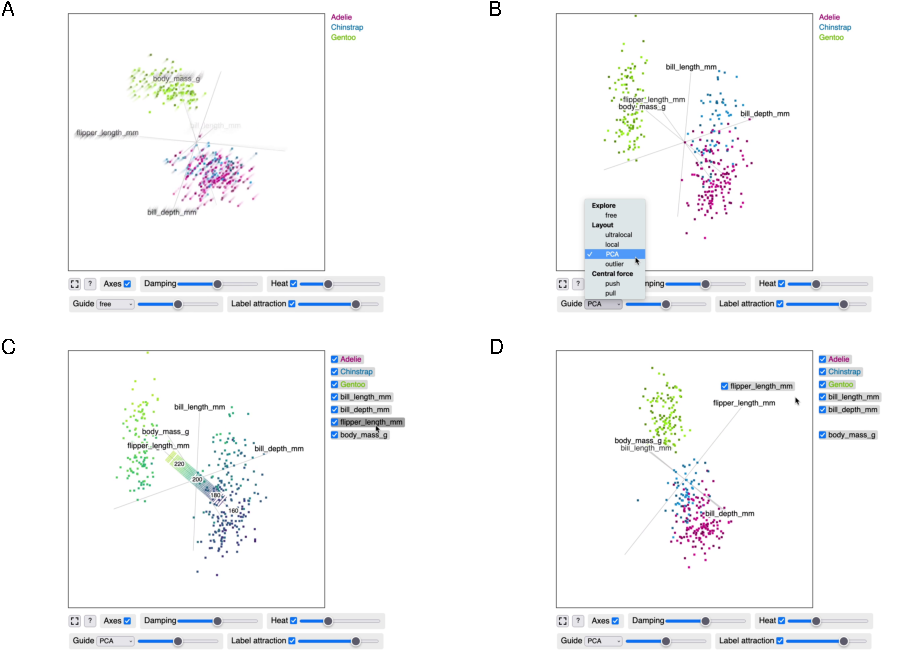
\includegraphics{RJ-2023-046_files/figure-latex/penguins-1.pdf}
\caption{\label{fig:penguins}\CRANpkg{palmerpenguins} data visualized using \CRANpkg{langevitour}. Each dot is a penguin, and the axes are four different penguin measurements. An interactive version of this figure is available in the supplemental file \texttt{figures-page.html}. (A) The widget initially spins at random. (B) The user has selected the PCA guide, and the widget has rotated to an informative projection using this guide. (C) The user has moused over a label, causing points to be colored by that variable. (D) The user has dragged a label onto the plot to concentrate on a particular variable.}
\end{figure}

The widget displays a moving projection of high-dimensional points onto a two-dimensional plane. The current projection is indicated using a collection of axis lines, with the axes labelled by their respective variable names. A second set of variable and group labels appear to the right of the plot area when interacting with the plot. These can be dragged on to the plot to control the projection. Let us now step through some manipulations the \CRANpkg{langevitour} widget allows.

\begin{itemize}
\item
  Setting a ``guide'' using the drop-down list. This causes \CRANpkg{langevitour} to pursue projections near the minimum of an energy function. For example, the PCA guide seeks projections with large variance in both the x and y directions.
\item
  Hiding particular groups by unchecking their checkbox in order to focus on other groups. For example by hiding Gentoo penguins, we can focus on the difference between Adelie and Chinstrap penguins. The guide is also only applied to the visible groups.
\item
  Hiding particular axes by unchecking their checkbox. For example, without bill length Adelie and Chinstrap penguins can no longer be distinguished.
\item
  Dragging labels onto the plot to concentrate on particular axes or try to separate a particular group. The projection may not exactly match the label positions since it must still be orthonormal.
\item
  Adjusting the damping slider. High damping produces jerky Brownian motion. Less damping produces smoother, less random motion. An intermediate damping level is the fastest way to explore the space of projections thoroughly.
\item
  Adjusting the heat slider. More heat makes the projection move faster, and stray further from the optimum projection defined by a guide or any labels dragged onto the plot.
\item
  When the mouse is over a group label the group is highlighted.
\item
  When the mouse is over an axis label a scale and rug are displayed, and points are colored according to their position on that axis.
\end{itemize}

Unchecking all but two or three axes can make the relationship between those particular axes clear. With three axes checked, the eye interprets the display as three-dimensional. A systematic way to examine a dataset is to proceed through all possible combinations of two or three axes.

If a particular interesting projection is found using \CRANpkg{langevitour} it can be brought back into R by pressing the ``?'' button and copying and pasting R code that is shown. The ``?'' button also shows a JSON record of the current settings of the widget, including form inputs and label positions. All or some of these settings can be specified to a future call to \texttt{langevitour()}, or applied to a running widget using Javascript code. Example code to control the widget using HTML buttons and Javascript is given in the supplemental file \texttt{figures-page.Rmd}.

\hypertarget{method}{%
\section{Method}\label{method}}

Say we have a set of \(n\) \(p\)-dimensional data points. A \(2 \times p\) projection matrix from \(p\) to 2 dimensions will be denoted \(\mathbf X\). The two rows of \(\mathbf X\) are called a 2-frame. These rows must be unit vectors and orthogonal to each other. The set of all 2-frames in \(p\) dimensions is a Stiefel manifold.

It will often be necessary to consider all of the elements of the projection matrix concatenated together into a single vector (``melted''), which will be denoted \(\mathbf x\). We will think of \(\mathbf x\) as a simulated physical system's ``position'' vector. With \(\mathbf x\) in use as the position of the system, the data points will be called the vectors \(\mathbf y_i\). The projection of point \(i\) into two dimensions is calculated with the matrix product \(\mathbf X \mathbf y_i\).

\hypertarget{langevindynamics}{%
\subsection{Langevin Dynamics overview}\label{langevindynamics}}

Projections are generated using a numerical simulation of Langevin Dynamics but with projections constrained to lie on the Stiefel manifold. This section \emph{briefly} summarizes Langevin Dynamics. The next section will describe the numerical simulation method and how the constraint is applied.

The description of Langevin Dynamics given here follows Leimkuhler and Matthews (2015), but for simplicity I set the Boltzmann constant to 1 and all masses to 1. We define a system with a position vector \(\mathbf x\) and a velocity vector \(\mathbf v\). We must specify a temperature \(T\), a damping rate \(\gamma\), and a potential energy function \(U(\mathbf x)\). The behavior of the system is then defined by a pair of Stochastic Differential Equations (SDEs):

\begin{align}
\mathrm{d}\mathbf{v} &= 
    -\gamma \mathbf{v} \mathrm{d}t 
    + \sqrt{2\gamma T}\mathrm{d}\mathbf{W} 
    -\nabla U(\mathbf{x}) \mathrm{d}t
    \label{eq:dv}\\
\mathrm{d}\mathbf{x} &= \mathbf{v} \mathrm{d}t
    \label{eq:dx}
\end{align}

Here \(\mathbf W\) is a vector of Wiener processes. For any positive time-step \(\Delta t\):

\[
\mathbf W(t+\Delta t) - \mathbf W(t) \sim \sqrt{\Delta t} \mathcal N(0,\mathbf I)
\]

The total energy of the system, kinetic energy plus potential energy, is called the Hamiltonian:

\begin{equation*}
H(\mathbf{x},\mathbf{v}) = \frac{1}{2}|\mathbf{v}|^2 + U(\mathbf{x})
\end{equation*}

In Equation \eqref{eq:dv} in a physical system, the first two terms would describe the exchange of kinetic energy with the surrounding environment. In the first term, kinetic energy is lost (damping), while the second term adds randomness to the velocity, increasing the kinetic energy again. The third term applies acceleration according to the gradient of the potential energy function.

If we were to set \(\gamma=0\), we would be doing Hamiltonian Dynamics, and the system's total energy would remain constant. If \(\gamma>0\) the total energy can fluctuate, and in the long run the process is ergodic (Leimkuhler and Matthews 2015 in section 6.4.4), producing samples with the Gibbs-Boltzmann probability density:

\begin{equation*}
\rho(\mathbf{x},\mathbf{v}) \propto e^{ -H(\mathbf{x},\mathbf{v})/T }
\end{equation*}

From this density, it can be seen that each component of the velocity is normally distributed with variance \(T\) and that the position has probability density

\begin{equation*}
\rho(\mathbf{x}) \propto e^{ -U(\mathbf{x})/T }
\end{equation*}

The potential energy function completely controls the distribution of positions being produced, providing a great deal of freedom. Here, we will use this to craft suitable potential energy functions to allow the user to control the explored projections.

\hypertarget{langevin-tour-numerical-simulation}{%
\subsection{Langevin Tour numerical simulation}\label{langevin-tour-numerical-simulation}}

We are to generate a sequence of animation frames \(i=1,2,...\), each with a projection matrix \(\mathbf X_i\) (written \(\mathbf x_i\) when viewed as a vector). Each frame will also have a velocity vector \(\mathbf v_i\). The time-step between frames can vary depending on the computational load from \CRANpkg{langevitour} and other things happening in the web browser. Call the time-step from frame \(i-1\) to frame \(i\) \(\Delta t_i\).

The Position Based Dynamics method (PBD, Müller et al. 2007) is used to perform the numerical simulation while constraining the system to produce orthonormal projection matrices. PBD is simple to implement and emphasizes stability over accuracy when enforcing constraints, which is appropriate and adequate for this application. Using PBD, in each iteration we will:

\begin{enumerate}
\def\labelenumi{\arabic{enumi}.}
\tightlist
\item
  Update the velocity.
\item
  Update the position based on the velocity.
\item
  Fix the updated position to be an orthonormal projection matrix.
\item
  Fix the velocity to be consistent with the fixed position.
\end{enumerate}

\hypertarget{step-1.-update-the-velocity}{%
\subsubsection{Step 1. Update the velocity}\label{step-1.-update-the-velocity}}

We will write \(\mathbf v'_i\) and \(\mathbf x'_i\) for the initially proposed velocity and position of the current frame. These will be adjusted in steps 3 and 4 to produce the final position and velocity, \(\mathbf x_i\) and \(\mathbf v_i\). The first step is to calculate

\begin{equation}
\mathbf v'_i = 
  e^{-\gamma \Delta t_i} \;  \mathbf v_{i-1} 
  + \sqrt{ T \left(1-e^{-2 \gamma \Delta t_i}\right) } \; \mathbf r_i 
  - \Delta t_i \; \nabla U(\mathbf x_{i-1})
  \label{eq:deltav}
\end{equation}

where the components of \(\mathbf r_i\) follow a standard normal distribution.

In the limit for \(\Delta t_i \rightarrow 0\), Equation \eqref{eq:deltav} matches the rate of change of the mean and rate of added variance in equation \eqref{eq:dv}. Equation \eqref{eq:deltav} has also been carefully chosen to have stable behavior for large \(\Delta t\) or \(\gamma\) or both. The first term decays the existing velocity by a factor of \(e^{-\gamma \Delta t_i}\). If Equation \eqref{eq:dv} only contained the first term, this would be the exact solution. This decay reduces the variance of the velocity by a factor of \(\left( e^{-\gamma \Delta t_i} \right) ^2\). The second term re-injects variance sufficient to restore the variance of the velocity in every direction (orthogonal to constraints) as \(T\).

A small refinement is made to avoid random rotation in the plane of projection, as this can be unsettling to view. Any part of the random noise \(\mathbf r_i\) within the plane of the projection is subtracted out before the noise is added to the velocity. More precisely, considering the noise in matrix form \(\mathbf R_i\) in the same way as the projection matrix \(\mathbf X_{i-1}\), the projection of each row of \(\mathbf R_i\) onto each row of \(\mathbf X_{i-1}\) is subtracted from that row of \(\mathbf R_i\). Previous tour software has also avoided this type of rotation, but in a different way, by using a ``geodesic interpolation'' method that operates between planes rather than frames (see Buja et al. 2005).

\hypertarget{step-2.-update-the-position-based-on-the-velocity}{%
\subsubsection{Step 2. Update the position based on the velocity}\label{step-2.-update-the-position-based-on-the-velocity}}

The position is advanced according to the velocity and the size of the time-step.

\begin{equation*}
\mathbf x'_i = \mathbf x_{i-1} + \Delta t_i \mathbf v'_i
\end{equation*}

\hypertarget{step-3.-fix-the-updated-position-to-be-an-orthonormal-projection-matrix}{%
\subsubsection{Step 3. Fix the updated position to be an orthonormal projection matrix}\label{step-3.-fix-the-updated-position-to-be-an-orthonormal-projection-matrix}}

Position Based Dynamics requires the proposed position \(\mathbf x'_i\) be projected back to a constraint-satisfying position \(\mathbf x_i\). Here, the constraint is \(\mathbf x_i\) represents an orthonormal projection matrix. Doing this arbitrarily might cause unexpected spinning in the projection plane. We must find the \emph{nearest} valid \(\mathbf x_i\) to \(\mathbf x'_i\).

Considering the proposed position vector as a projection matrix, we take the singular value decomposition and set the singular values to 1.

\begin{align}
\mathbf U \mathbf S \mathbf V^\top & = \mathbf X'_i 
    \label{eq:svd} \\
\mathbf X_i & = \mathbf U \mathbf V^\top
    \label{eq:orthonormalize}
\end{align}

Here, \(\mathbf U\) is a \(2\times 2\) orthonormal matrix, \(\mathbf S\) is a \(2\times 2\) diagonal matrix, and \(\mathbf V\) is a \(p\times 2\) matrix with orthonormal columns. Let \(s_j\) be the values along the diagonal of \(\mathbf S\), the singular values, all of which are non-negative.

Equation \eqref{eq:orthonormalize} chooses the closest orthonormal projection matrix in terms of Euclidean distance to \(\mathbf{x'}_i\).
Stated another way, this is the matrix \(\mathbf X\) that minimizes the Frobenius norm \(\|\mathbf X' - \mathbf X\|\) with the proposed projection matrix \(\mathbf X'\).
To see this, consider first the problem of finding the nearest orthonormal projection matrix to
\(\mathbf{ U^\top X' }\).

\[
\mathbf{ U^\top X' = U^\top USV^\top =SV^\top }
\]

For each row in
\(\mathbf{ U^\top X' }\),
\(\mathbf{\left(U^\top X' \right)}_{j,\cdot} = s_j \mathbf V^\top_{j,\cdot}\),
the nearest unit vector will be parallel to this vector, namely
\(\mathbf V^\top_{j,\cdot}\).
We know that the rows of
\(\mathbf V^\top\) are orthogonal, so
\(\mathbf V^\top\) is the nearest orthonormal projection matrix to
\(\mathbf{U^\top X' }\).
Multiplying both matrices by an orthonormal matrix does not change the Frobenius norm of their difference, so the nearest orthonormal projection matrix to
\(\mathbf{UU^\top X' = X'}\) is
\(\mathbf{UV^\top}\).

\hypertarget{step-4.-fix-the-velocity-to-be-consistent-with-the-fixed-position}{%
\subsubsection{Step 4. Fix the velocity to be consistent with the fixed position}\label{step-4.-fix-the-velocity-to-be-consistent-with-the-fixed-position}}

Position Based Dynamics requires the velocity to match the actual update made to the position, rather than the initially proposed update.

\begin{equation*}
\mathbf v_i = \frac{\mathbf x_i - \mathbf x_{i-1}}{\Delta t_i}
\end{equation*}

\hypertarget{guiding-projections-using-the-potential-energy-function}{%
\subsection{Guiding projections using the potential energy function}\label{guiding-projections-using-the-potential-energy-function}}

We can use any function we like for the potential energy \(U(\mathbf x)\), so long as we can calculate its gradient. This is used in \CRANpkg{langevitour} to provide a set of automatic guides and also as a method of interaction.

When an energy function is being used, the temperature \(T\) plays a role analogous to variance in the normal distribution. When the temperature is very low, the system seeks the minimum of the energy function. As the temperature is raised, projections further and further from the minimum are produced.

\hypertarget{linear-energy-function-for-interaction}{%
\subsubsection{Linear energy function for interaction}\label{linear-energy-function-for-interaction}}

For some choice of vector \(\mathbf a\), we can set the energy function to be the dot product

\begin{equation*}
U(\mathbf x) = - \mathbf a \mathbf x
\end{equation*}

This encourages the projection to have a large component parallel to \(\mathbf a\). In \CRANpkg{langevitour} this is used when labels are dragged onto the plot area to control the placement of particular axes of the high-dimensional space or to control the position of the mean of a group of points.

\hypertarget{central-force-energy-function}{%
\subsubsection{Central force energy function}\label{central-force-energy-function}}

The Box-Cox power transformation (Box and Cox 1964) provides a useful building block for energy functions.

\[
f(x ; \lambda_1 , \lambda_2) = 
\begin{cases}
 \dfrac{(x + \lambda_2)^{\lambda_1} - 1}{\lambda_1} & \text{if } \lambda_1 \neq 0, \\
 \ln (x + \lambda_2) & \text{if } \lambda_1 = 0
\end{cases}
\]

An energy function creating forces away from or toward the center can be defined using:

\[
U_\text{central}(\mathbf x ; c,\lambda_1,\lambda_2) = \frac{c}{n} \sum_{i=1}^n f\left(|\mathbf X \mathbf y_{i}|^2 ; \lambda_1,\lambda_2\right)
\]

\CRANpkg{langevitour} offers a central ``push'' guide (\(c<0,\lambda_1=0.5,\lambda_2=0.0001\)) and a central ``pull'' guide (\(c>0,\lambda_1=0.5,\lambda_2=0.0001\)). These cone-shaped energy functions result in a nearly constant magnitude outward or inward force on points, except for a small region close to the center.

\hypertarget{layout-by-point-point-repulsion}{%
\subsubsection{Layout by point-point repulsion}\label{layout-by-point-point-repulsion}}

It was found that repulsion forces between pairs of points can be used to produce an informative layout. Let \(S\) be a set of pairs of points \((i,j)\). Ideally we would make this the set of all possible pairs of points but, for computational efficiency, \CRANpkg{langevitour} uses a random mini-batch of 5,000 pairs of points per iteration, with a different mini-batch used each time. Using random mini-batches to approximate the gradient injects extra noise into the system (see Mandt, Hoffman, and Blei 2017). The effect is similar to increasing the temperature slightly.

\[
U_\text{layout}(\mathbf x ; \lambda_1,\lambda_2) = 
    \frac{c}{|S|} \sum_{(i,j) \in S} f\left(|\mathbf X \mathbf y_{j}-\mathbf X \mathbf y_{i}|^2; \lambda_1,\lambda_2\right)
\]

The power parameter \(\lambda_1\) determines whether the layout is governed by long-range or short-range forces. \CRANpkg{langevitour} offers ``ultra-local'' (\(c<0,\lambda_1=-1,\lambda_2=0.0025\)), ``local'' (\(c<0,\lambda_1=0,\lambda_2=0.0001\)), ``PCA'' (\(c<0,\lambda_1=1,\lambda_2=0\)), and ``outlier'' (\(c<0,\lambda_1=2,\lambda_2=0\)) guides. The ``local'' guide is the preferred default. With this guide, pairs of points that are near to each other exert more force than pairs of points that are far apart. The ``ultra-local'' guide potentially produces better layouts but is somewhat unstable. The ``PCA'' guide is equivalent to PCA. The ``outlier'' guide seeks projections where there are some points that are very far from other points.

\hypertarget{blending-energy-functions}{%
\subsubsection{Blending energy functions}\label{blending-energy-functions}}

A sum of energy functions such as the above can be used to produce behavior that blends the behaviors from the individual functions. For example, there could be an active guide and also one or more labels dragged onto the plot.

\hypertarget{implementation}{%
\section{Implementation}\label{implementation}}

\CRANpkg{langevitour} uses the \CRANpkg{htmlwidgets} framework. It was an important design goal that using \CRANpkg{langevitour} be no more difficult than any other plotting function in R. \CRANpkg{htmlwidgets} allows Javascript widgets to be used in most places that conventional R graphical output can be used. The widget may be displayed during an interactive R session or included in a knitted document with a call to the \texttt{langevitour} function. The only required argument is a matrix (or data frame) of numerical data. A grouping of rows is often also given, allowing points to be distinguished by color. There are further optional arguments providing adjustments to the scaling, appearance, and further optional features.

The \CRANpkg{htmlwidgets} \texttt{scaffoldWidget} function was used to scaffold the package, including functions to create the widget (\texttt{langevitour}) and to use the widget in \CRANpkg{shiny} applications (\texttt{langevitourOutput}, \texttt{renderLangevitour}).

\CRANpkg{langevitour} operates without a server, so the R portion of \CRANpkg{langevitour} is limited to sanity-checking all the inputs and ensuring \CRANpkg{htmlwidgets} will translate the data to JSON consistently. In particular, vectors convert to lists, which ensures vectors of length 1 are not unboxed. A Javascript class performs calculation, plotting, and interaction. The D3 Javascript package is used to perform drag-and-drop interaction, color operations, scale operations, and some DOM element manipulation. The SVD-JS Javascript package is used for the singular value decomposition calculation. The jStat Javascript package is used to produce normally distributed random numbers. Besides these packages, calculations are performed using plain Javascript code, following the steps in the previous section.

Gradients need to be calculated in order to use potential energy functions as a guides or for interaction. The necessary partial derivatives were found by hand, and used to implement a collection of gradient functions. To add a new guide, a function to calculate the required gradient can be written, and the source code edited to make it available in the widget interface.

In Javascript, animation frames are scheduled using \texttt{requestAnimationFrame}, allowing the browser to manage the frame rate, co-ordinate multiple animations within a document, and pause animation when the document is not on screen. A typical frame rate for the browser to aim for is 60 frames per second. The frame rate may drop if there is too much calculation and drawing required, such as when there are many points to display. Multiple widgets may be active in a document at once, and even if the document is visible, not all widgets may be visible. To minimize CPU usage the animation is paused if a widget scrolls off-screen or is otherwise hidden. Canvas-based rendering was used.

\hypertarget{scrna-seq-example}{%
\section{scRNA-Seq example}\label{scrna-seq-example}}

A dataset by Kang et al. (2018) demonstrates many of the complex high-dimensional features that are found in scRNA-Seq data. In this dataset, peripheral blood mononuclear cells (PBMCs) from eight patients with lupus were pooled. PBMCs are cells from the immune system that circulate in blood, including monocytes, B cells, T cells, and natural killer (NK) cells. These cells were then stimulated with a cytokine, recombinant interferon beta, causing a change in the gene expression of the cells. The dataset contains a sample of unstimulated cells (U), and a separate sample of stimulated cells (S).

Single cell sequencing produces a small proportion of doublets, where two cells end up in a single micro-droplet and appear in the final data as a single cell. A nice feature of this dataset is that doublets containing cells from two different individuals can be identified with certainty due to genetic differences between the individuals.

\hypertarget{processing-steps}{%
\subsection{Processing steps}\label{processing-steps}}

Sequencing data was produced using a 10x Chromium Single Cell instrument and an Illumina HiSeq 2500 sequencer. Kang et al. (2018) then processed sequencing reads using the 10x Genomics CellRanger software and provided the resulting RNA molecule count data in the Gene Expression Omnibus (GEO) database as accession number GSE96583. They also provided their annotation of the cells into different types, and doublet detection based on genetic differences between individuals. Slightly simplified annotations are shown in this article. There are 29,065 cells in total. 3,169 of these are identified as doublets.

In the processed data for each of the two samples, there is a matrix giving the number of molecules of RNA associated with each gene within each cell. Normalization by total count per cell, log transformation, and PCA were carried out using the \CRANpkg{Seurat} package (Hoffman 2022). As per Seurat defaults, only the top 2,000 highly variable genes are used. Each resulting Principal Component (PC) has a score for each cell and a loading for each gene.

The top PCs capture as much variation in the data as possible but are not necessarily individually interpretable. To aid biological interpretation, it would be better if each component represented changes in the expression of a distinct set of genes. Each differentially expressed gene should have loadings that are mostly concentrated in a single component, and we prefer the loadings to be positive if possible. With these goals in mind, the varimax rotation of the gene loadings was found using the \texttt{varimax()} function in the built-in stats package, with Kaiser normalization disabled. Both the gene loadings and the cell scores are rotated. Then, for each component, if the loadings have negative skew both the loadings and scores are negated.

Genetic differences can not identify doublets containing cells from the same individual, so Bioconductor package \BIOpkg{scDblFinder} (Germain et al. 2022) was used to impute further doublets using the \texttt{recoverDoublets()} function. This only works between cells of different types, but doublets containing cells of the same type are not a problem. A further 595 doublets were identified this way.

The dataset was sub-sampled down to 10,000 cells to allow a smooth frame rate in \CRANpkg{langevitour},

The R code used to process the scRNA-Seq data is given in the supplemental file \texttt{processing.R}. Code for figure generation from the processed data is given in \texttt{figures.R}.

\hypertarget{cell-scores}{%
\subsection{Cell scores}\label{cell-scores}}

Results from analysis with \CRANpkg{Seurat} are shown in Figure~\ref{fig:standard}. The scree plot has a fat tail with no clear elbow. A large number of PCs potentially contain useful information. The top 10 PCs will be used simply as a manageable number with which to interact. Common practice is to visualize cells using a 2D UMAP layout computed from the PCs, as shown in Figure~\ref{fig:standard}B, to see what clusters exist in the data and try to understand their relationships.

\begin{figure}
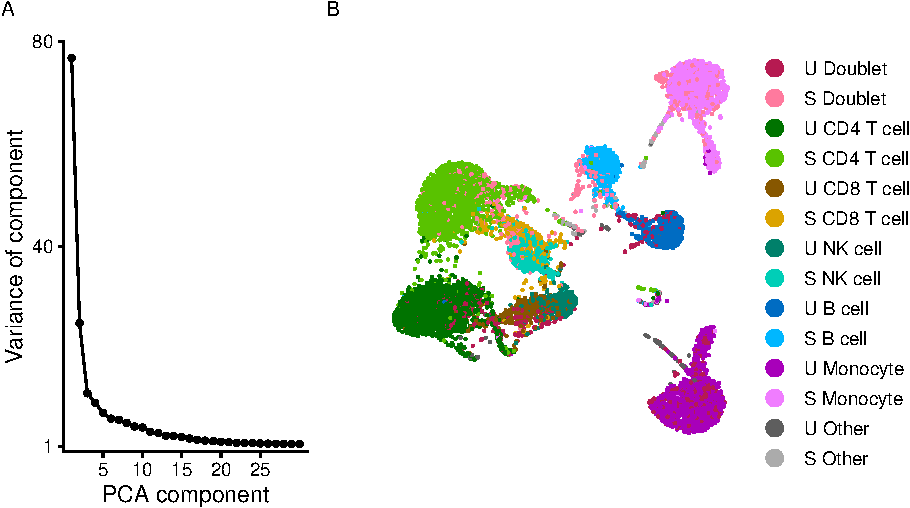
\includegraphics{RJ-2023-046_files/figure-latex/standard-1} \caption{scRNA-Seq analysis using Seurat. (A) A scree plot showing variance accounted for by each PC. The scree plot has a fat tail, indicating that variation in the data can not be summarized with only a few PCs. (B) UMAP layout based on the cell scores of the first 10 PCs. U are unstimulated and S are stimulated cells.}\label{fig:standard}
\end{figure}

UMAP (McInnes, Healy, and Melville 2018) is a non-linear dimensionality reduction technique. Ironically, UMAP may give a curvy biological appearance to linear structures in the original data! Problems with UMAP are discussed by Coenen and Pearce (2019). They are similar to the problems with t-SNE (Wattenberg, Viégas, and Johnson 2016), an earlier method that UMAP has largely supplanted for scRNA-Seq analysis. Problems include that UMAP may arbitrarily change the distances between clusters and that UMAP will hide whether clusters are more or less spread-out by design.

Figure \ref{fig:raw} shows the \CRANpkg{langevitour} visualization of the cell scores. Components have been varimax rotated to improve interpretability (see previous section). With \CRANpkg{langevitour}, we only ever see linear projections of the data. Straight lines remain straight, and parallelograms remain parallelograms. Distances may be decreased but will not be increased by the projection.

\begin{figure}
\centering
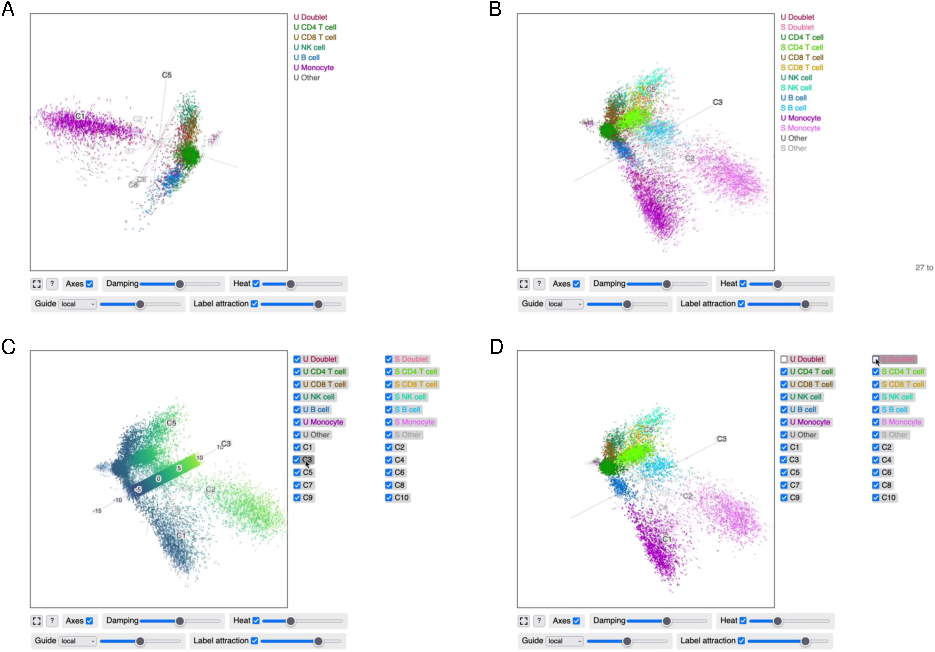
\includegraphics{RJ-2023-046_files/figure-latex/raw-1.pdf}
\caption{\label{fig:raw}scRNA-Seq cell scores visualized using langevitour. An interactive version of this figure is available in the supplemental file \texttt{figures-page.html}. The ``local'' guide is active. (A) Unstimulated cells. (B) All cells. (C) Colored by component 3. (D) Doublets hidden.}
\end{figure}

This is a moderately complex dataset. We will step through some manipulations of the widget in Figure~\ref{fig:raw} to try to understand it better.

\begin{itemize}
\item
  To simplify the dataset, hide the stimulated cells by unticking the checkbox on all the ``S'' labels.
\item
  To find a projection giving a good overview of the relationships between unstimulated PBMC cells, activate the ``local'' guide from the drop-down list. The guided layout may not be able to perfectly separate all the clusters as UMAP can. However, small relative motions make clear where clusters are overlapping by accident rather than real proximity. For example, B cells and T cells are distinct.
\item
  Examine the scale by mousing over the labels for particular axes. The scale for each component is meaningful, representing distance along a certain direction in scaled gene expression space. The direction is specified by the gene loadings, which are examined in a section \protect\hyperlink{geneloadings}{below}.
\item
  Mouse over the ``U Doublet'' and ``S Doublet'' labels to highlight doublets. Doublets located between two clusters may be interpreted as a mixture of a pair of cells with different cell types. Hiding the doublets by unchecking their checkboxes makes the clusters more distinct.
\end{itemize}

Let us compare this data view to the UMAP layout (Figure~\ref{fig:standard}B). In the linear view provided by langevitour, the monocytes are more spread out than other cell clusters. This isn't visible in UMAP which, as a deliberate feature, erases differences in scale. The whiskers extending from various clusters in the UMAP correspond to components at right angles to other components in the data, i.e., a subset of cells in which certain genes are active. For example, the thin whiskers extending from the unstimulated and stimulated monocytes extend in the same direction, along C7, but in the UMAP they extend in different directions. Doublets in the UMAP tend to form clumps near the edges of clusters or between clusters. In the linear data view, they are spread out between clusters.

\hypertarget{k-nearest-neighbor-denoising}{%
\subsubsection{k-nearest neighbor denoising}\label{k-nearest-neighbor-denoising}}

\begin{figure}
\centering
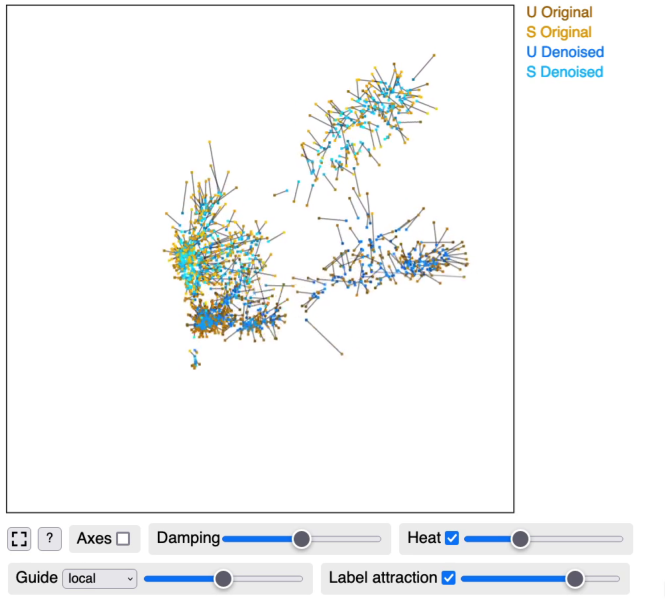
\includegraphics{RJ-2023-046_files/figure-latex/denoising-1.pdf}
\caption{\label{fig:denoising}Noise reduction of scRNA-Seq cell scores. Original and denoised positions of 1,000 cells are shown, joined by lines. An interactive version of this figure is available in the supplemental file \texttt{figures-page.html}.}
\end{figure}

The fuzziness of the clusters in Figure \ref{fig:raw} is an honest depiction of the data. However, to interpret the geometry of the data, it may be helpful to reduce the amount of noise. We want to do so with minimal distortion. A suggested method is implemented in \CRANpkg{langevitour} in the function \texttt{knnDenoise()}, based on the k-nearest neighbor graph. The k-nearest neighbors to each point are first found. Then, each point is updated to be the average of the set of points reachable within a certain number of steps along the directed k-nearest neighbors graph. Here \(k=30\) and two steps were used. This method is loosely inspired by the k-nearest neighbors smoothing method of Wagner, Yan, and Yanai (2018) and the use of the nearest neighbor graph in UMAP.

A comparison of the original and denoised cell positions is shown in Figure~\ref{fig:denoising} for a sample of 1,000 cells. The effect has been to make clusters thinner and smaller but not to move them in space. The full result is shown in Figure~\ref{fig:denoised}.

\begin{figure}
\centering
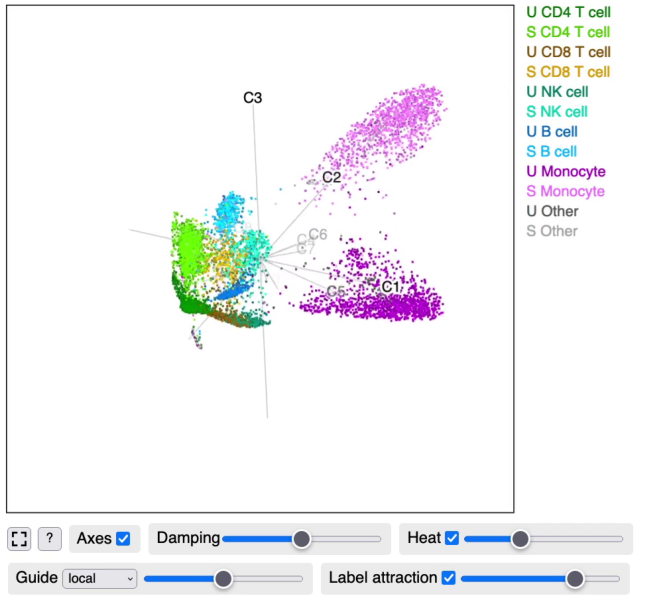
\includegraphics{RJ-2023-046_files/figure-latex/denoised-1.pdf}
\caption{\label{fig:denoised}Noise reduced scRNA-Seq cell scores.}
\end{figure}

We will again step through some widget manipulations, to understand the relationships between clusters and components.

\begin{itemize}
\item
  To provide an overview of the data, the ``local'' guide has already been activated.
\item
  Doublets still lie between clusters in this denoised version. Compare this to the UMAP layout, where the doublets tend to be attached to one or other clusters. To make the clusters cleaner, hide the doublets by unticking the checkboxes on the doublet labels.
\item
  To examine component C1, drag the C1 label on to the plot. This pulls out the monocyte cluster. It appears monocytes are associated with C1.
\item
  To undo this action, drag the C1 label to the right to remove it from the plot area.
\end{itemize}

Similarly
C5
pulls out CD8 T cells and NK cells, and
C6
pulls out B cells.
The response to the cytokine is mostly contained in
C3
with a further monocyte specific response in
C2.

\hypertarget{geneloadings}{%
\subsection{Gene loadings}\label{geneloadings}}

Each component examined in the preceding sections represents a certain pattern of gene expression. These patterns of gene expression are represented by the gene loadings. Within each component, each gene has a loading. As will be seen, the tendency is for large loadings to be concentrated in a relatively small set of genes for each component. Genes with large loadings may provide insights into the biology represented by each component based on their known function or involvement in known biological pathways.

The gene loadings may also be examined using \CRANpkg{langevitour}, as shown in Figure \ref{fig:gene}. In this figure, the points are genes, and the variables are the loading for each component.

\begin{figure}
\centering
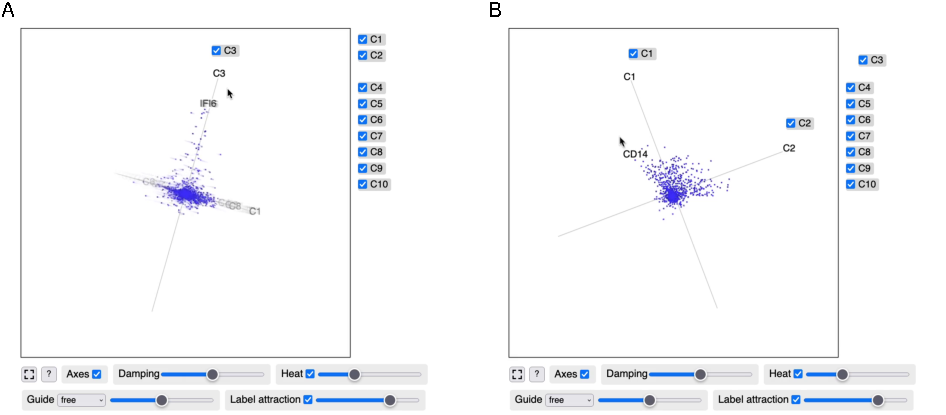
\includegraphics{RJ-2023-046_files/figure-latex/gene-1.pdf}
\caption{\label{fig:gene}scRNA-Seq gene loadings visualized using langevitour. The points are genes and the variables are the loading for each component. An interactive version of this figure is available in the supplemental file \texttt{figures-page.html}. (A) Genes involved in component 3. (B) Genes involved in components 1 and 2.}
\end{figure}

\begin{itemize}
\item
  Observe the widget spinning freely for a while. The overall geometry is of a spiky ball. The spikes generally represent sets of genes with large loadings in one component.
\item
  Drag particular component labels onto the plot to examine them. Biological phenomena such as different cell types (C5, C6) or responses to the cytokine (C3)
  often involve distinct sets of genes. Furthermore, cell types are defined more by genes' activation than genes' deactivation. Varimax rotation was able to align these distinct sets of genes into specific components. An exception is genes used by monocytes and the monocyte response to stimulation (C1 and C2). These two components show a broad fan of genes, which can be interpreted as the genes involved in being a monocyte also being involved to varying degrees in the monocyte response to stimulation.
\item
  Mouse near points to see the specific genes they represent.
\end{itemize}

\hypertarget{discussion}{%
\section{Discussion}\label{discussion}}

Langevin Dynamics produces samples from a specified probability distribution and produces a path suitable for animation. Besides tours, a possible future application would be to use this to visualize uncertainty in the posterior distribution of a Bayesian statistical model while placing details of the model directly under interactive control. Visualization of samples from a distribution has been previously investigated by Hullman, Resnick, and Adar (2015), as the Hypothetical Outcome Plots (HOPs) method. HOPs displays a graphical representation of samples from a multivariate distribution one after the other. An appealing feature of HOPs is that any visualization may be used. The viewer can perceive the uncertainty in the distribution, and how the variables relate to each other in the values they might take. However the display of HOPs simply hops from one sample to the next. There is also earlier work in geospatial applications, such as by Ehlschlaeger, Shortridge, and Goodchild (1997) in which a smooth animation was produced by interpolating between a sequence of samples. They note that interpolated frames may no longer follow the original distribution, and propose a method that preserves the correct variance in interpolated frames for their specific application. By using Langevin Dynamics, a smooth animation could be produced in which each individual frame is naturally drawn from the correct distribution.

Langevin Dynamics is similar to the Hamiltonian Monte Carlo method (HMC, see Neal 2011) used for example by the Stan software package (Carpenter et al. 2017). Usually HMC alternates steps of completely randomizing the velocity and relatively long runs of Hamiltonian Dynamics simulation. This would produce a continuous path, but with occasional sharp turns. Neal (2011) describes a version of HMC with frequent partial velocity refreshment that more closely resembles Langevin Dynamics. An accept/reject step can make the sampling precisely accurate even with discrete time-steps. Another possibility, for large datasets, is to use mini-batch gradients for computational efficiency (Mandt, Hoffman, and Blei 2017). Mini-batch gradients provide a noisy estimate of the full gradient and, with careful tuning, the level of noise required for Langevin Dynamics will be injected into the velocity. It may be possible to animate sampling from complex models in real-time smoothly.

Motion provides a channel of visual information not possible in static images. We are not accustomed to visualizing objects in more than three dimensions, but things that move together in the natural environment are usually physically connected, and this seems to be how our eyes interpret the small rotations in more than three dimensions displayed by \CRANpkg{langevitour}.

A Javascript widget has been introduced for interactively exploring high-dimensional data. It is readily usable from the R environment, Shiny websites, or HTML documents generated using R Markdown, including static HTML reports, slideshows, and journal articles.

\hypertarget{acknowledgements}{%
\section{Acknowledgements}\label{acknowledgements}}

The idea for \CRANpkg{langevitour} arose during discussions with Prof.~Di Cook and Dr.~Stuart Lee at Monash University.

\hypertarget{references}{%
\section*{References}\label{references}}
\addcontentsline{toc}{section}{References}

\hypertarget{refs}{}
\begin{CSLReferences}{1}{0}
\leavevmode\vadjust pre{\hypertarget{ref-Asimov1985}{}}%
Asimov, Daniel. 1985. {``{The Grand Tour}: A Tool for Viewing Multidimensional Data.''} \emph{SIAM Journal on Scientific and Statistical Computing} 6 (1): 128--43. \url{https://doi.org/10.1137/0906011}.

\leavevmode\vadjust pre{\hypertarget{ref-Box1964}{}}%
Box, G E P, and D R Cox. 1964. {``An Analysis of Transformations.''} \emph{Journal of the Royal Statistical Society. Series B (Methodological)} 26: 211--52. \url{http://www.jstor.org/stable/2984418}.

\leavevmode\vadjust pre{\hypertarget{ref-Buja2005}{}}%
Buja, Andreas, Dianne Cook, Daniel Asimov, and Catherine Hurley. 2005. {``Computational Methods for High-Dimensional Rotations in Data Visualization.''} In \emph{Data Mining and Data Visualization}, edited by C R Rao, E J Wegman, and J L Solka, 24:391--413. Elsevier. \url{https://doi.org/10.1016/S0169-7161(04)24014-7}.

\leavevmode\vadjust pre{\hypertarget{ref-Carpenter2017}{}}%
Carpenter, Bob, Andrew Gelman, Matthew D. Hoffman, Daniel Lee, Ben Goodrich, Michael Betancourt, Marcus Brubaker, Jiqiang Guo, Peter Li, and Allen Riddell. 2017. {``{Stan}: A Probabilistic Programming Language.''} \emph{Journal of Statistical Software} 76. \url{https://doi.org/10.18637/jss.v076.i01}.

\leavevmode\vadjust pre{\hypertarget{ref-Coenen2019}{}}%
Coenen, Andy, and Adam Pearce. 2019. {``Understanding {UMAP}.''} \url{https://pair-code.github.io/understanding-umap/}.

\leavevmode\vadjust pre{\hypertarget{ref-Cook1995}{}}%
Cook, Dianne, Andreas Buja, Javier Cabrera, and Catherine Hurley. 1995. {``{Grand Tour} and {Projection Pursuit}.''} \emph{Journal of Computational and Graphical Statistics} 4 (September): 155--72. \url{https://doi.org/10.1080/10618600.1995.10474674}.

\leavevmode\vadjust pre{\hypertarget{ref-Ehlschlaeger1997}{}}%
Ehlschlaeger, Charles R., Ashton M. Shortridge, and Michael F. Goodchild. 1997. {``Visualizing Spatial Data Uncertainty Using Animation.''} \emph{Computers \& Geosciences} 23 (May): 387--95. \url{https://doi.org/10.1016/S0098-3004(97)00005-8}.

\leavevmode\vadjust pre{\hypertarget{ref-Germain2022}{}}%
Germain, Pierre-Luc, Aaron Lun, Will Macnair, and Mark D. Robinson. 2022. {``Doublet Identification in Single-Cell Sequencing Data Using {scDblFinder}.''} \emph{F1000Research} 10 (May): 979. \url{https://doi.org/10.12688/f1000research.73600.2}.

\leavevmode\vadjust pre{\hypertarget{ref-Hart2022}{}}%
Hart, Casper, and Earo Wang. 2022. \emph{Detourr: Portable and Performant Tour Animations}. \url{https://CRAN.R-project.org/package=detourr}.

\leavevmode\vadjust pre{\hypertarget{ref-Hoffman2022}{}}%
Hoffman, Paul. 2022. \emph{{Seurat}: Tools for Single Cell Genomics}. \url{https://CRAN.R-project.org/package=Seurat}.

\leavevmode\vadjust pre{\hypertarget{ref-Horst2020}{}}%
Horst, Allison Marie, Alison Presmanes Hill, and Kristen B Gorman. 2020. \emph{Palmerpenguins: {Palmer Archipelago (Antarctica)} Penguin Data}. \url{https://allisonhorst.github.io/palmerpenguins/}.

\leavevmode\vadjust pre{\hypertarget{ref-Hullman2015}{}}%
Hullman, Jessica, Paul Resnick, and Eytan Adar. 2015. {``{Hypothetical} {Outcome} {Plots} Outperform Error Bars and Violin Plots for Inferences about Reliability of Variable Ordering.''} \emph{PLOS ONE} 10 (November): e0142444. \url{https://doi.org/10.1371/journal.pone.0142444}.

\leavevmode\vadjust pre{\hypertarget{ref-Kang2018}{}}%
Kang, Hyun Min, Meena Subramaniam, Sasha Targ, Michelle Nguyen, Lenka Maliskova, Elizabeth McCarthy, Eunice Wan, et al. 2018. {``Multiplexed Droplet Single-Cell {RNA-sequencing} Using Natural Genetic Variation.''} \emph{Nature Biotechnology} 36 (1): 89--94. \url{https://doi.org/10.1038/nbt.4042}.

\leavevmode\vadjust pre{\hypertarget{ref-Leimkuhler2015}{}}%
Leimkuhler, Ben, and Charles Matthews. 2015. \emph{Molecular Dynamics with Deterministic and Stochastic Numerical Methods}. 1st ed. Interdisciplinary Applied Mathematics, 39.

\leavevmode\vadjust pre{\hypertarget{ref-Lemons1997}{}}%
Lemons, Don S., and Anthony Gythiel. 1997. {``{Paul Langevin}'s 1908 Paper {{`On the Theory of Brownian Motion'} {[}{`Sur La Théorie Du Mouvement Brownien,'} C. R. Acad. Sci. (Paris) 146, 530-533 (1908){]}}.''} \emph{American Journal of Physics} 65 (November): 1079--81. \url{https://doi.org/10.1119/1.18725}.

\leavevmode\vadjust pre{\hypertarget{ref-Mandt2017}{}}%
Mandt, Stephan, Matthew D Hoffman, and David M Blei. 2017. {``{Stochastic Gradient Descent} as {Approximate Bayesian Inference}.''} \emph{Journal of Machine Learning Research} 18: 1--35. \url{http://jmlr.org/papers/v18/17-214.html}.

\leavevmode\vadjust pre{\hypertarget{ref-McInnes2018}{}}%
McInnes, Leland, John Healy, and James Melville. 2018. {``{UMAP: Uniform Manifold Approximation and Projection} for Dimension Reduction.''} \emph{arXiv}. \url{https://doi.org/10.48550/ARXIV.1802.03426}.

\leavevmode\vadjust pre{\hypertarget{ref-Muller2007}{}}%
Müller, Matthias, Bruno Heidelberger, Marcus Hennix, and John Ratcliff. 2007. {``Position Based Dynamics.''} \emph{Journal of Visual Communication and Image Representation} 18 (2): 109--18. \url{https://doi.org/10.1016/j.jvcir.2007.01.005}.

\leavevmode\vadjust pre{\hypertarget{ref-Neal2011}{}}%
Neal, Radford M. 2011. {``{MCMC} Using {Hamiltonian Dynamics}.''} In \emph{Handbook of {Markov Chain Monte Carlo}}, edited by Steve Brooks, Andrew Gelman, Galin Jones, and Xiao-Li Meng, 113--62. CRC Press.

\leavevmode\vadjust pre{\hypertarget{ref-Swayne1998}{}}%
Swayne, Deborah F., Dianne Cook, and Andreas Buja. 1998. {``{XGobi}: Interactive Dynamic Data Visualization in the {X Window System}.''} \emph{Journal of Computational and Graphical Statistics} 7 (1): 113--30. \url{https://doi.org/10.1080/10618600.1998.10474764}.

\leavevmode\vadjust pre{\hypertarget{ref-Vaidyanathan2021}{}}%
Vaidyanathan, Ramnath, Yihui Xie, JJ Allaire, Joe Cheng, Carson Sievert, and Kenton Russell. 2021. \emph{Htmlwidgets: {HTML} Widgets for {R}}. \url{https://CRAN.R-project.org/package=htmlwidgets}.

\leavevmode\vadjust pre{\hypertarget{ref-Wagner2018}{}}%
Wagner, Florian, Yun Yan, and Itai Yanai. 2018. {``K-Nearest Neighbor Smoothing for High-Throughput Single-Cell {RNA-Seq} Data.''} \emph{bioRxiv}, April, 217737. \url{https://doi.org/10.1101/217737}.

\leavevmode\vadjust pre{\hypertarget{ref-Wattenberg2016}{}}%
Wattenberg, Martin, Fernanda Viégas, and Ian Johnson. 2016. {``How to Use {t-SNE} Effectively.''} \emph{Distill} 1 (October). \url{https://doi.org/10.23915/distill.00002}.

\leavevmode\vadjust pre{\hypertarget{ref-Wickham2011}{}}%
Wickham, Hadley, Dianne Cook, Heike Hofmann, and Andreas Buja. 2011. {``Tourr: An {R} Package for Exploring Multivariate Data with Projections.''} \emph{Journal of Statistical Software} 40. \url{https://doi.org/10.18637/jss.v040.i02}.

\end{CSLReferences}


\address{%
Paul Harrison\\
Monash Genomics and Bioinformatics Platform, Monash University\\%
15 Innovation Walk\\ Monash University, Clayton Campus\\ Clayton VIC, Australia, 3800\\
%
\url{https://logarithmic.net/pfh/}\\%
\textit{ORCiD: \href{https://orcid.org/0000-0002-3980-268X}{0000-0002-3980-268X}}\\%
\href{mailto:paul.harrison@monash.edu}{\nolinkurl{paul.harrison@monash.edu}}%
}
